\section{ÉLABORATION D'UN MODÈLE CINÉMATIQUE}\TLSectionLabel{4}

\subsection{Démarche}

\subsubsection*{Étape 1 — Identifier les classes d'équivalence cinématique}

Repérer les pièces ne présentant aucun mouvement relatif, les colorier,
nommer les CEC \(S_0,S_1,\ldots\) et lister les pièces qui les constituent.

\begin{center}
\begin{minipage}{.57\linewidth}
\begin{itemize}
  \item exclure les pièces déformables : ressorts, joints, rondelles élastiques ;
  \item exclure les éléments roulants : billes, rouleaux, aiguilles ;
  \item choisir un bâti unique, considéré fixe dans le référentiel d'étude.
\end{itemize}
\end{minipage}\hfill
\begin{minipage}{.38\linewidth}\centering
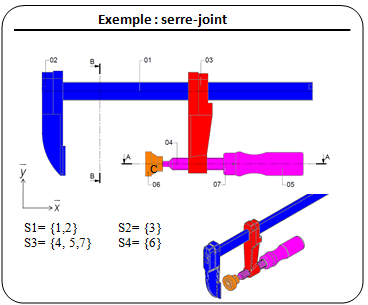
\includegraphics[width=\linewidth,height=.22\textheight,keepaspectratio]{images/image80.png}
\end{minipage}
\end{center}

\subsubsection*{Étape 2 — Réaliser le graphe des liaisons}

\begin{itemize}
  \item représenter chaque CEC par une bulle ;
  \item identifier le bâti ;
  \item identifier les contacts et les mouvements relatifs ;
  \item relier les bulles et préciser le nom et les éléments géométriques des liaisons.
\end{itemize}

\TLImageSmall[.55\linewidth]{images/image84.png}

Deux questions guident l'identification : quelle est la nature des surfaces
en contact ? Quels sont les mouvements relatifs possibles ?

\subsubsection*{Étape 3 — Élaborer le schéma cinématique}

Positionner les centres et les axes, placer les symboles normalisés avec le
code couleur, relier les éléments de même couleur et vérifier la cohérence
avec les mouvements réels.

\TLImageSmall[.60\linewidth]{images/image3.png}

\begin{TLRemark}
Lorsque le graphe a été simplifié grâce aux liaisons équivalentes, le schéma
obtenu est un \textbf{schéma cinématique minimal}.
\end{TLRemark}

\subsubsection*{Application : micromoteur}

Le micromoteur comporte quatre CEC : le carter \(0\), le vilebrequin \(1\),
la bielle \(2\) et le piston \(3\).

\begin{center}
\begin{minipage}[t]{.47\linewidth}\centering
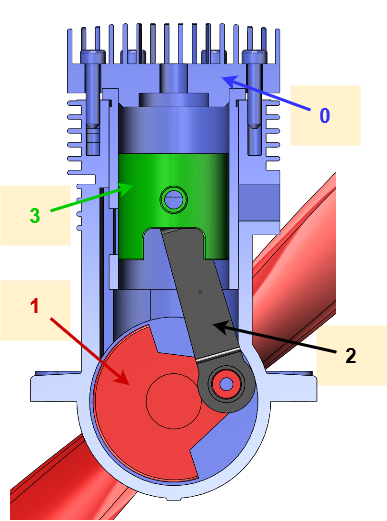
\includegraphics[width=.92\linewidth,height=.28\textheight,keepaspectratio]{images/image86.png}\\
\emph{Identification des CEC et points caractéristiques}
\end{minipage}\hfill
\begin{minipage}[t]{.47\linewidth}\centering
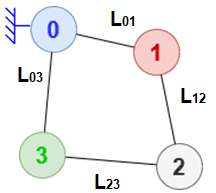
\includegraphics[width=.88\linewidth,height=.28\textheight,keepaspectratio]{images/image87.png}\\
\emph{Graphe des liaisons}
\end{minipage}
\end{center}

Les liaisons sont :
\[
L_{01}\text{ pivot en }A,\quad
L_{12}\text{ pivot en }B,\quad
L_{23}\text{ pivot glissant en }C,\quad
L_{30}\text{ pivot glissant en }A.
\]

\TLImageSmall[.55\linewidth]{images/image93.png}

\subsection{Modélisation des guidages}

Grâce à des éléments glissants ou roulants, on obtient des mouvements
relatifs plus performants du point de vue énergétique.

\begin{tabularx}{\linewidth}{|>{\centering\arraybackslash}p{.32\linewidth}|X|}
\hline
\rowcolor{gray!25}\textbf{Coussinets} & \textbf{Modélisation}\\ \hline

\includegraphics[width=.74\linewidth]{images/image95.png}\quad
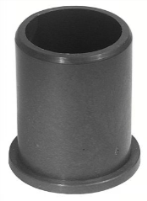
\includegraphics[width=.74\linewidth]{images/image96.png}
& Liaison pivot ou pivot glissant.\\ \hline
\end{tabularx}

\subsubsection*{Roulements}

Le choix entre pivot et sphérique dépend notamment de l'angle maximal de
rotulage. Le jeu interne autorise de faibles rotations autour des axes
secondaires.

\begin{tabularx}{\linewidth}{|>{\centering\arraybackslash}X|>{\centering\arraybackslash}X|}
\hline
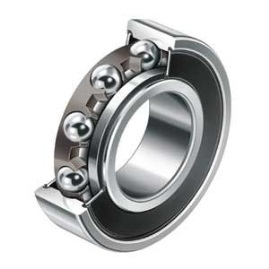
\includegraphics[width=.43\linewidth]{images/image99.jpeg}\quad
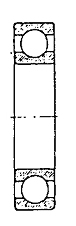
\includegraphics[width=.18\linewidth]{images/image100.jpeg}
&
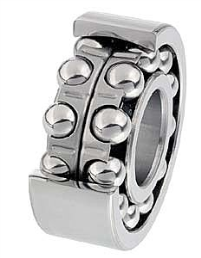
\includegraphics[width=.43\linewidth]{images/image101.png}\quad
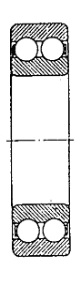
\includegraphics[width=.18\linewidth]{images/image102.jpeg}\\
Une rangée de billes : en général rotulage \(>5'\), modèle sphérique.
&
Deux rangées de billes : en général rotulage \(<5'\), modèle pivot.\\ \hline
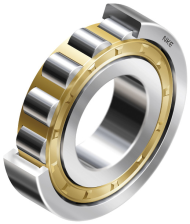
\includegraphics[width=.43\linewidth]{images/image103.png}\quad

\includegraphics[width=.30\linewidth]{images/image104.png}
&

\includegraphics[width=.43\linewidth]{images/image106.jpeg}\quad

\includegraphics[width=.18\linewidth]{images/image107.jpeg}\\
Aiguilles ou rouleaux : rotulage \(<5'\), modèle pivot.
&
Roulement à rotule : rotulage de \(2^\circ\) à \(4^\circ\), modèle sphérique.\\ \hline
\end{tabularx}

\begin{tabularx}{\linewidth}{|>{\bfseries}p{.30\linewidth}|X|}
\hline
Pivot & rotulage \(<5'\) et deux bagues arrêtées en translation.\\ \hline
Pivot glissant & rotulage \(<5'\) et une bague libre en translation.\\ \hline
Sphérique & rotulage \(>5'\) et deux bagues arrêtées en translation.\\ \hline
Sphère-cylindre & rotulage \(>5'\) et une bague libre en translation.\\ \hline
\end{tabularx}

\subsubsection*{Autres guidages}

\begin{tabularx}{\linewidth}{|>{\centering\arraybackslash}p{.34\linewidth}|X|}
\hline

\includegraphics[width=.72\linewidth]{images/image108.png}
& \textbf{Douille à billes :} pivot glissant.\\ \hline
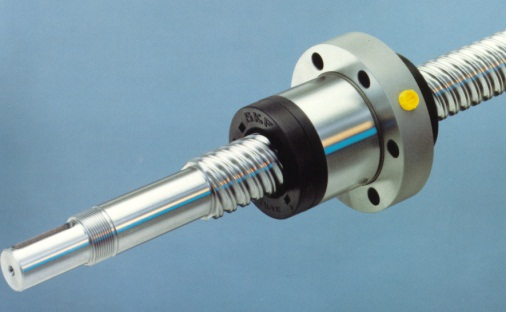
\includegraphics[width=.72\linewidth]{images/image110.jpeg}
& \textbf{Vis à billes :} hélicoïdale.\\ \hline
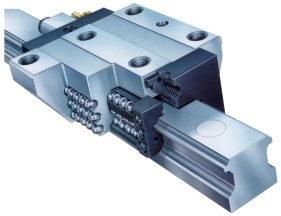
\includegraphics[width=.72\linewidth]{images/image111.jpeg}
& \textbf{Guidage à billes :} glissière.\\ \hline

\includegraphics[width=.36\linewidth]{images/image112.png}\quad
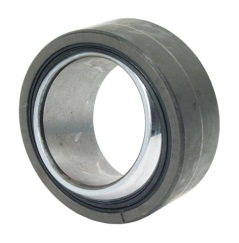
\includegraphics[width=.36\linewidth]{images/image113.jpeg}
& \textbf{Rotule lisse :} sphérique.\\ \hline
\end{tabularx}

\subsection{Modélisation des transmetteurs usuels}

\begin{tabularx}{\linewidth}{|>{\centering\arraybackslash}p{.32\linewidth}|>{\centering\arraybackslash}X|}
\hline
\rowcolor{gray!20}\textbf{Réalisation technologique} & \textbf{Schéma cinématique}\\ \hline
\textbf{Roue et vis sans fin}\\
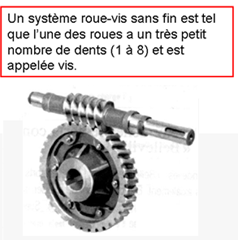
\includegraphics[width=.72\linewidth]{images/image115.png}
& 
\includegraphics[width=.70\linewidth]{images/image114.png}\\ \hline
\textbf{Poulie-courroie}\\
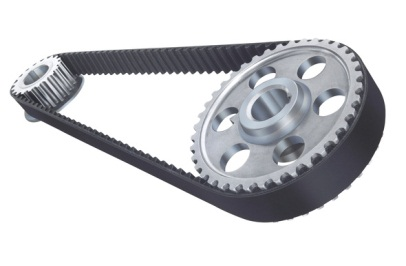
\includegraphics[width=.72\linewidth]{images/image117.jpeg}
& 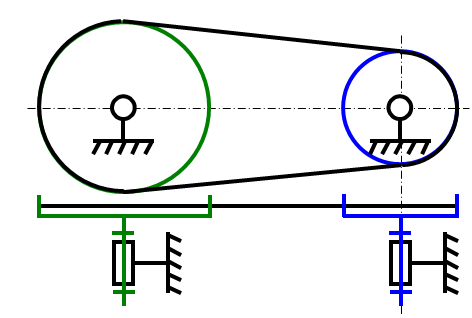
\includegraphics[width=.70\linewidth]{images/image116.png}\\ \hline
\textbf{Engrenages}\\

\includegraphics[width=.72\linewidth]{images/image119.png}
& 
\includegraphics[width=.70\linewidth]{images/image118.png}\\ \hline
\end{tabularx}

% -----------------------------------------------------------------------------
\section{PARAMÉTRAGE D'UN SCHÉMA CINÉMATIQUE}\TLSectionLabel{5}

Afin de simuler le comportement du mécanisme, on associe une base orthonormée
directe à chaque CEC. Le solide \(i\) reçoit le repère
\(\mathcal R_i=(O_i,\vec x_i,\vec y_i,\vec z_i)\).

\begin{center}
\begin{minipage}[t]{.48\linewidth}\centering

\includegraphics[width=.92\linewidth,height=.28\textheight,keepaspectratio]{images/image120.png}\\
\emph{Antenne parabolique}
\end{minipage}\hfill
\begin{minipage}[t]{.48\linewidth}\centering

\includegraphics[width=.92\linewidth,height=.28\textheight,keepaspectratio]{images/image121.png}\\
\emph{Échelle EPAS}
\end{minipage}
\end{center}

\subsection{Base orthonormée}

Une base associée à un solide est :
\begin{itemize}
  \item \textbf{orthonormée} : vecteurs orthogonaux deux à deux et unitaires ;
  \item \textbf{directe} : orientation donnée par la règle de la main droite.
\end{itemize}

\TLImageSmall[.34\linewidth]{images/image124.jpeg}

Les bases se déplacent avec les CEC. On utilise des paramètres de mouvement :
un angle pour une liaison pivot et une distance pour une glissière.

\subsection{Figures de changement de base}

Pour construire une figure de changement de base :
\begin{enumerate}
  \item dessiner un petit angle, de l'ordre de \(20^\circ\) ;
  \item placer face à soi le vecteur commun autour duquel la base tourne ;
  \item compléter les deux bases de manière directe ;
  \item reporter les égalités entre vecteurs unitaires.
\end{enumerate}

\TLImageSmall[.42\linewidth]{images/image125.jpeg}

Il faut une figure par liaison pivot. Lorsque plusieurs pivots ont des axes
parallèles, les figures peuvent être superposées.

\TLReflectionBox{Réaliser les figures de changement de base de l'antenne parabolique et de l'échelle EPAS, puis celles du robot de soudage.}

\begin{center}
\begin{minipage}[t]{.43\linewidth}\centering
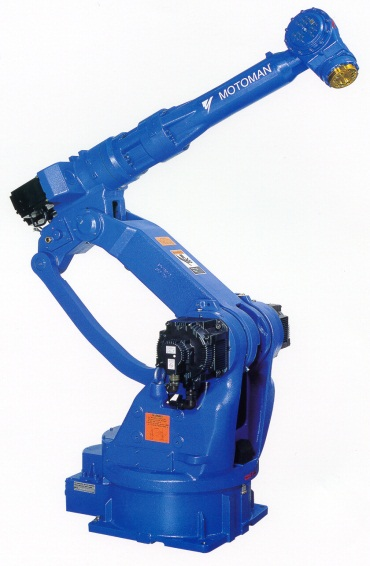
\includegraphics[width=.84\linewidth,height=.26\textheight,keepaspectratio]{images/image140.jpeg}\\
\emph{Robot de soudage}
\end{minipage}\hfill
\begin{minipage}[t]{.53\linewidth}\centering
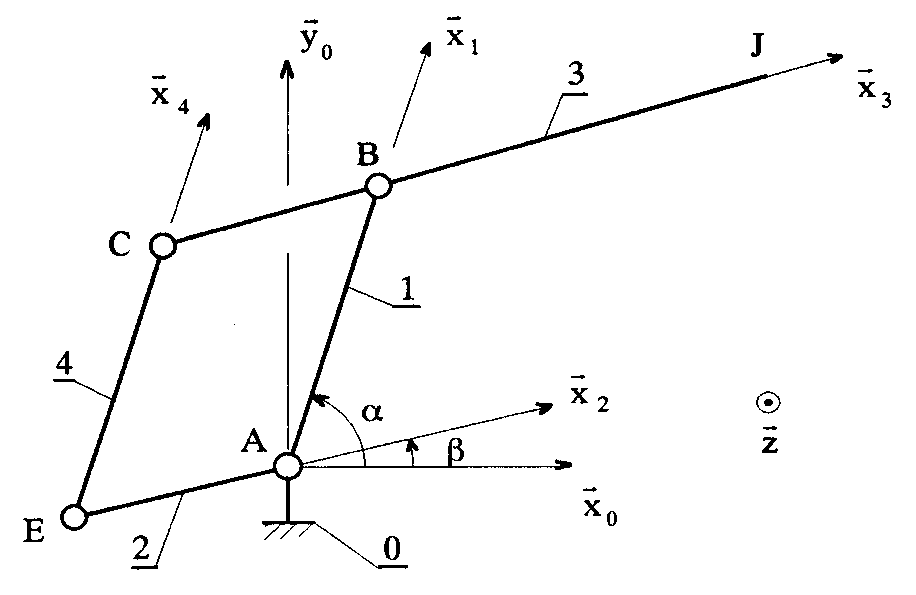
\includegraphics[width=\linewidth,height=.26\textheight,keepaspectratio]{images/image139.png}\\
\emph{Paramétrage du mécanisme}
\end{minipage}
\end{center}

% -----------------------------------------------------------------------------
\section{LIAISON ÉQUIVALENTE}\TLSectionLabel{6}

Une liaison équivalente à plusieurs liaisons entre deux CEC traduit le même
mouvement relatif et permet de transmettre les mêmes actions mécaniques.

\subsection{Analyse des mouvements possibles}

La démarche intuitive est la suivante :
\begin{enumerate}
  \item identifier chaque liaison ;
  \item déterminer ses degrés de liberté prise isolément ;
  \item partir de la liaison qui possède le moins de degrés de liberté ;
  \item tester les mouvements encore possibles avec l'association ;
  \item identifier la liaison équivalente et ses éléments géométriques.
\end{enumerate}

\TLImageSmall[.66\linewidth]{images/image149.png}

\subsection{Liaisons en parallèle avec les torseurs}

Les liaisons \(L_1,\ldots,L_n\) sont en parallèle lorsqu'elles relient
directement les mêmes solides \(S_1\) et \(S_2\).

\begin{center}
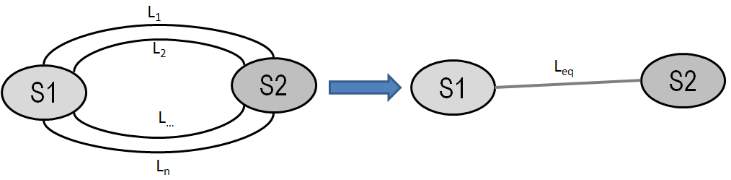
\includegraphics[width=.50\linewidth,height=.15\textheight,keepaspectratio]{images/image151.png}
\[
\left\{\mathcal V_{2/1}^{L_{\mathrm{eq}}}\right\}
=
\left\{\mathcal V_{2/1}^{L_1}\right\}
=
\left\{\mathcal V_{2/1}^{L_2}\right\}
=\cdots=
\left\{\mathcal V_{2/1}^{L_n}\right\}.
\]
\end{center}

Le torseur de la liaison équivalente doit être compatible avec tous les
torseurs des liaisons en parallèle.

\subsection{Liaisons en série avec les torseurs}

Les liaisons sont en série lorsqu'elles sont disposées à la suite les unes
des autres par l'intermédiaire de \(n-1\) CEC.

\begin{center}
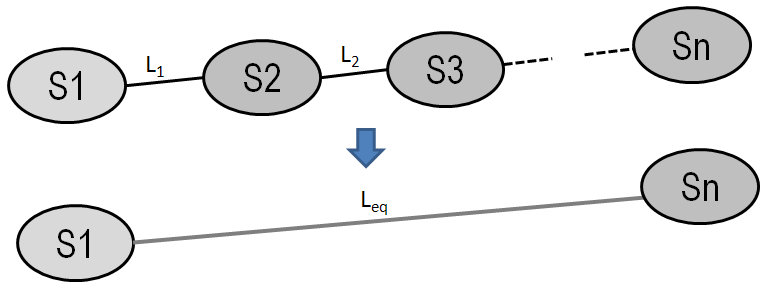
\includegraphics[width=.50\linewidth,height=.15\textheight,keepaspectratio]{images/image153.png}
\[
\left\{\mathcal V_{n/1}^{L_{\mathrm{eq}}}\right\}
=
\left\{\mathcal V_{n/n-1}^{L_n}\right\}
+\cdots+
\left\{\mathcal V_{3/2}^{L_2}\right\}
+\left\{\mathcal V_{2/1}^{L_1}\right\}.
\]
\end{center}

La liaison équivalente présente les degrés de liberté qui n'ont été supprimés
par aucune des liaisons de la chaîne.

% -----------------------------------------------------------------------------
\section{Sources}\TLSectionLabel{7}

Ce cours reprend et organise des ressources provenant notamment de Jacques
Le Goff, Corentin Kerzreho, Stéphane Génouel, de documents industriels
publics et d'activités pédagogiques de collègues de l'UPSTI.
